\begin{sidewaysfigure}[htbp]
\centering 
  \subfloat[Low friction, average void fraction.]
  {
	  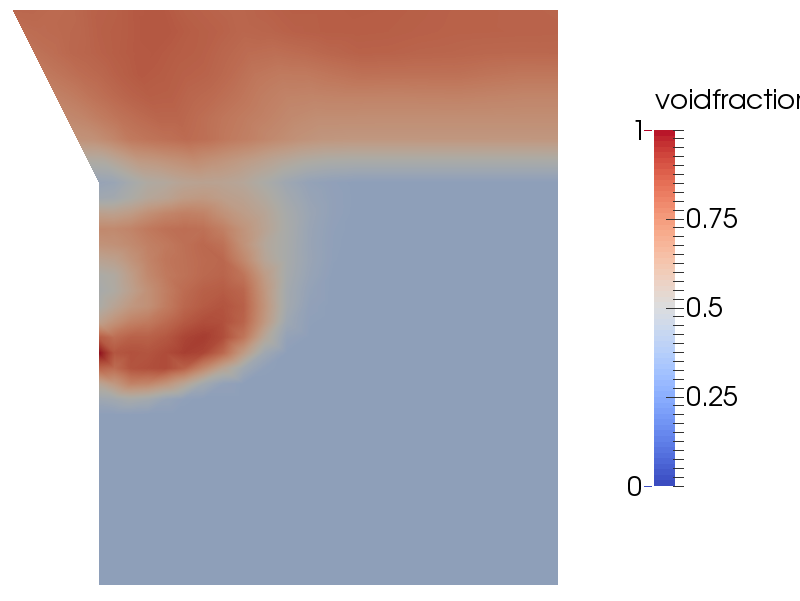
\includegraphics[width=.32\columnwidth]{images/235vf_average_lf}
	  \label{fig:235vf_average_lf}
  }
  \quad
    \subfloat[High friction, average void fraction.]
    {
	  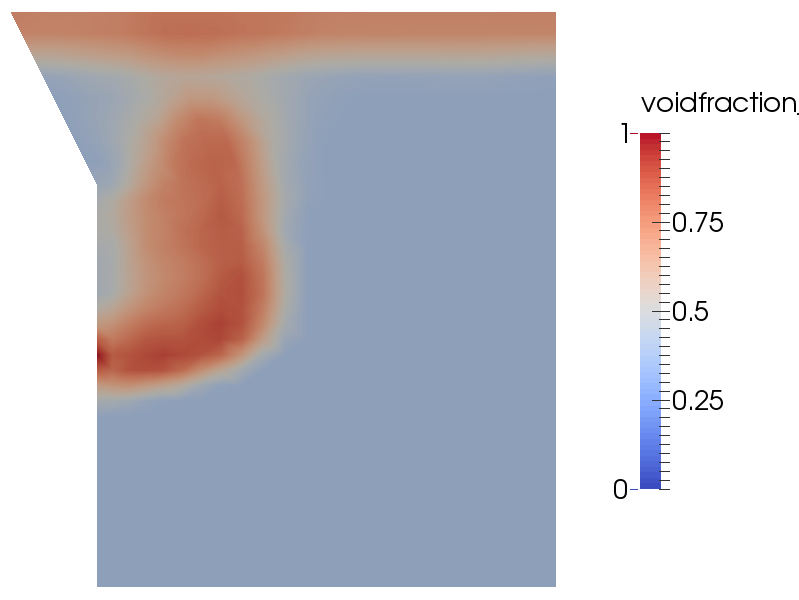
\includegraphics[width=.32\columnwidth]{images/234vf_average_hf}
	  \label{fig:234vf_average_hf}
  }
  \quad
    \subfloat[High friction, average void fraction.]
    {
	  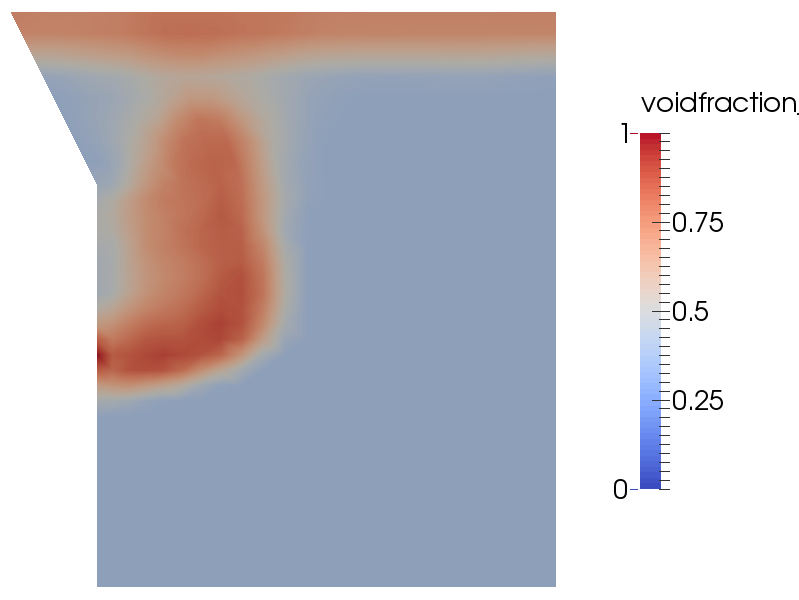
\includegraphics[width=.32\columnwidth]{images/234vf_average_hf}
	  \label{fig:234vf_average_hf}
  }
  \\
  \subfloat[Low friction, standard deviation void fraction.]
  {
	  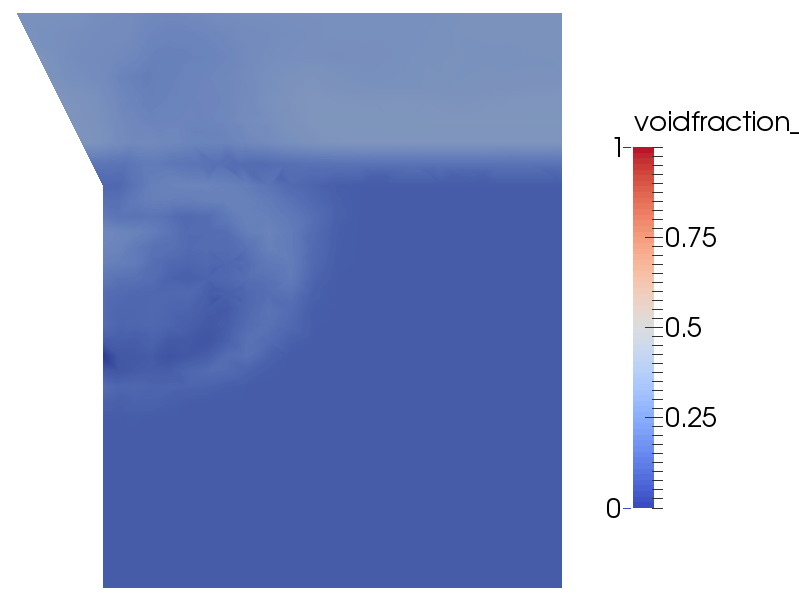
\includegraphics[width=.32\columnwidth]{images/237vf_std_lf}
	  \label{fig:237vf_std_lf}
  }
  \quad
    \subfloat[High friction, standard deviation void fraction.]
    {
	  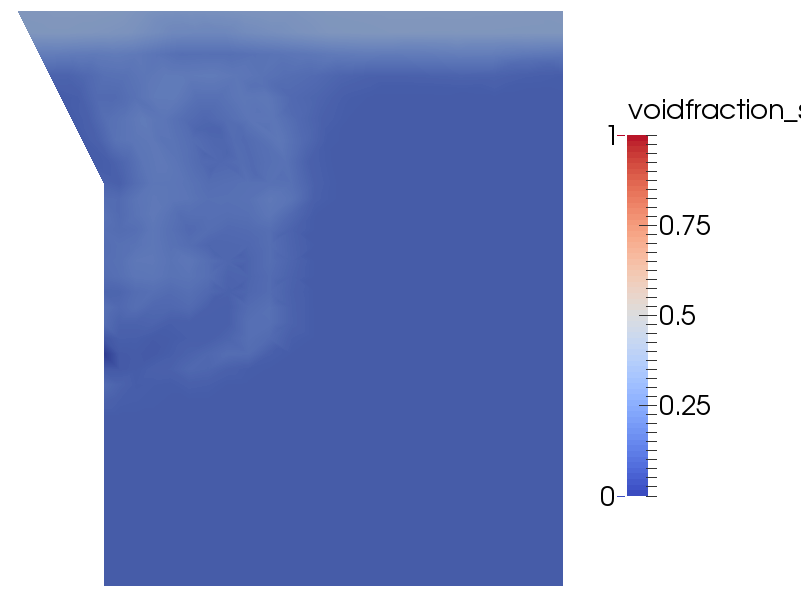
\includegraphics[width=.32\columnwidth]{images/236vf_std_hf}
	  \label{fig:236vf_std_hf}  }
  \\
  \caption{Void fraction with different sliding friction coefficient.}
  \label{fig:239racewayvf}
\end{sidewaysfigure}